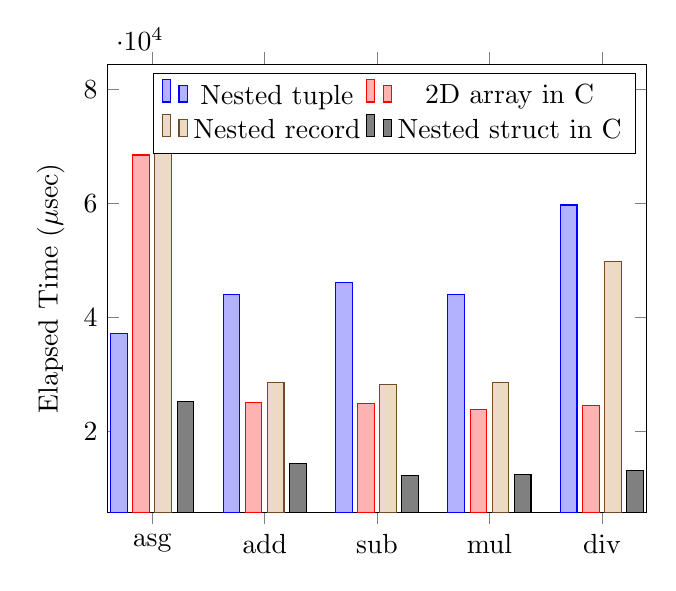
\begin{tikzpicture}
\begin{axis}[
  ybar, bar width=6pt,
  ylabel=Elapsed Time ($\mu$sec),
  symbolic x coords={asg, add, sub, mul, div},
  legend columns=2]
\addplot coordinates
  {(asg, 37227.6) (add, 43990.8) (sub, 46055.6) (mul, 43937.6) (div, 59695)};
\addplot coordinates
  {(asg, 68454.2) (add, 25028.8) (sub, 24933.2) (mul, 23775.2) (div, 24469.8)};
\addplot coordinates
  {(asg, 77836) (add, 28498) (sub, 28265.8) (mul, 28566.2) (div, 49820.6)};
\addplot coordinates
  {(asg, 25209.2) (add, 14292) (sub, 12311.4) (mul, 12413.6) (div, 13181)};
\legend{Nested tuple, 2D array in C, Nested record, Nested struct in C}
\end{axis}
\end{tikzpicture}
